% ------------------------------------------------------------------------
% ------------------------------------------------------------------------
% UFGRC: Modelo de Trabalho Acadêmico em conformidade com 
% ABNT NBR 14724:2011: Informação e documentação - Trabalhos acadêmicos -
% Apresentação
% ------------------------------------------------------------------------
% ------------------------------------------------------------------------

% Opções: 
%   Tipo do trabalho     = tcc1/tcc2
%   Situação do trabalho = pre-defesa/pos-defesa
% -- opções do pacote babel --
% Idioma padrão = brazil
	%english,			% idioma adicional para hifenização
	%brazil				% o último idioma é o PRINCIPAL do documento

\documentclass[tcc2, pos-defesa, english, brazil]{packages/ufgrc}

% ---------------------------------------------------------------------------
% Pacotes Opcionais
% ---------------------------------------------------------------------------
\usepackage{rotating}           % Usado para rotacionar o texto
\usepackage[all,knot,arc,import,poly]{xy}   % Pacote para desenhos gráficos
% Este pacote pode conflitar com outros pacotes gráficos como o ``pictex''
% Então é necessário usar apenas um dos pacotes conflitantes
\newcommand{\VerbL}{0.52\textwidth}
\newcommand{\LatL}{0.42\textwidth}
% ---------------------------------------------------------------------------


% ---
% Informações de dados para CAPA e FOLHA DE ROSTO
% ---
% Tanto na capa quanto nas folhas de rosto apenas a primeira letra da primeira palavra (ou nomes próprios) devem estar em letra maiúscula, todas as demais devem ser em letra minúscula.
\titulo{Arquitetura de Computadores}

\autor{ Marco Túlio Macedo Rodrigues,
        Pablo Vinicius da Silva,
        Vitor do Valde Bernardo }
        
\genero{M} % Gênero do autor (M = Masculino / F = Feminino)
\orientador[Orientadora]{Prof. Dr.}{Tércio Alberto dos Santos Filho}
\data{06}{2017} % Data da defesa
% ---

% Membros da banca examinadora
% - O primeiro membro será automaticamente o orientador
% - Caso haja coorientador, este será o segundo membro
% Nome dos demais membros e suas instituições


% ---
% RESUMOS
% ---

% Resumo em PORTUGUÊS
% conter no máximo 500 palavras
% conter no mínimo 1 e no máximo 5 palavras-chave (obrigatoriamente separadas por vírgula)

\textoresumo[brazil]{
    Este trabalho é desenvolvido para a disciplina de Arquitetura de Computadores pela Universidade Federal de Goiás. O trabalho visa no desenvolvimento de 3 projetos, onde cada projeto visa trazer conhecimentos em diferentes da área disciplina. Estaremos abordando diferentes temas: PWM, Sleep Mode, Comunicação SPI. 
    }{Arquitetura, Computadores, Microcontroladores, PWP, SPI}


% resumo em INGLÊS
% conter no máximo 500 palavras
% conter no mínimo 1 e no máximo 5 palavras-chave (obrigatoriamente separadas por vírgula)

\textoresumo[english]{
   This work is developed for a discipline of Computer Architecture by the Federal University of Goiás. The work aims at the development of 3 projects, where each project aims to bring knowledge in different disciplines area. We will be addressing different topics: PWM, Sleep Mode, SPI Communication.
    }{Architecture, Computer, Microcontrollers, PWP, SPI }
    
% ---
% Configurações de aparência do PDF final
% ---
\hypersetup{
	colorlinks=true     % false: boxed links; true: colored links
}
% --- 

% ----------------------------------------------------------
% ELEMENTOS PRÉ-TEXTUAIS
% ----------------------------------------------------------

% Inserir a ficha catalográfica
%\incluifichacatalografica*{tex/pre-textual/fichaCatalografica.pdf}
%\incluifichacatalografica

% DEDICATÓRIA / AGRADECIMENTO / EPÍGRAFE
\textodedicatoria*{tex/pre-textual/dedicatoria}
\textoagradecimentos*{tex/pre-textual/agradecimentos}
\textoepigrafe*{tex/pre-textual/epigrafe}

% Inclui a lista de figuras
\incluilistadefiguras

% Inclui a lista de tabelas
%\incluilistadetabelas

% Inclui a lista de quadros
%\incluilistadequadros

% Inclui a lista de algoritmos
%\incluilistadealgoritmos

% Inclui a lista de códigos
\incluilistadecodigos

% Inclui a lista de siglas e abreviaturas
\incluilistadesiglas

% Inclui a lista de símbolos
%\incluilistadesimbolos

% ----
% Início do documento
% ----
\begin{document}

% ----------------------------------------------------------
% ELEMENTOS TEXTUAIS
% ----------------------------------------------------------
\textual

\chapter{Introdução}
\label{chapter:introducao}
% Comando simples para exibir comandos Latex no texto
\newcommand{\comando}[1]{\textbf{$\backslash$#1}}


Neste trabalho serão apresentados alguns projetos que foram construídos sobre a linguagem C, utilizando de algumas funções específicas para uso em microcontroladores.

São projetos simples com o objetivo de simular o uso de protocolos e funções específicos, como por exemplo MLP (Modulação por lagura de pulso), uso de CPU em modo sleep mode e uso de interrupções, padrão \sigla{SPI}{Serial Peripheral Interface}.

O principal objetivo dos projetos é proporcionar a experiencia do aluno
trabalhar com os registradores direto para realização dos projetos. 3 temas básicos serão discutidos: \sigla{MLP}{Modulação por largura de puslo}, Modos de economizar a energia em circuito utilizando Sleep Mode, Formas de dois dispositivos se comunicarem utilizando o padrão \sigla{SPI}{Serial Peripheral Interface}.



\chapter{Proejeto 1: Fading LED}
\label{chapter:Fading LED}

Desenvolva um projeto que através de um potenciômetro aumente ou diminua a frequência de uma determina saída X utilizando PWM.

\section{O que é PWM ?}

A técnologia \sigla{PWM}{Pulse Width Modulation} ou no português Modulação de Largura de Pulso permite que os microcontroladores atenuem as luzes, controle a velocidade de motores e geram tensões análogicas.Isso é feito alterando o comprimento do pulso, permitidno assim a saída ser controlada.

Neste projeto iremos controlar a intesidade de brilho de um LED utilizando a \sigla{PINB0)}{saída} PWM do microncontralador: atmega8.

O pulso ocorre em uma frequência regular, neste caso na freqüência de modulação. Chamamos de \sigla{Dutty Cicle}{Ciclo de trabalho} a razão entre o tamanho do pulso pelo periodo de tempo. Logo, quanto maior é o tempo de trabalho maior também será a saída. Porntato, quando alteramos essa saída que alimenta o LED, alteramos  a intensidade do seu brilho também.

\begin{figure}[htb]
 \caption{Duty Cicle}
 \label{fig:Duty Cicle}
 \centering
 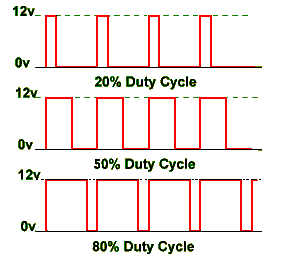
\includegraphics[scale=0.23]{Duty-Cycle.png}
 \fdireta{avrprojects:duty_cicle}
\end{figure}

\section{PWM no atmega8}

Todos os projetos aqui desenvolvidos serão utilizando o microcontrolador: ATMega8. Ele pode ser usado para gerar sinais PWM. Um microcontrolador como o ATMega8 tem três canais de hardware PWM a bordo do chip. Para o desenvolvimento deste trabalho estaremos utilizando o sinal PWM que está no pino PORTBO.

O PWM de hardware pode ser programado configurando os registradores do temporizador. O ATMega8 tem três registradores de temporizador que você precisa definir para programar o PWM:

\begin{enumerate}

\item O registrador TCCR1A deverá colocar o temporizador no modo PWM.
\item Os registradores TCNT1H e TCNT1Lsão usados para ajustar a freqüência de modulação
\item O registrador OCR1A é usado para ajustar o ciclo de trabalho.

\end{enumerate}

\section{Esquemático e Montagem}

O circuito consiste em ligar um microcontrolador ATMega8, onde que iremos ligar um LED conectador no pino PORTB0, através de um resistor de 220 ohm.

Pretendemos variar o brilho do LED através dos valores fornecidos pelo potênciometro conectado no pino PORTC0. Os valores serão lidos pela porta análogica do ATMega8, que neste caso se encontra no PORTC0.

Veja o esquematico da montagem na figura 2:

\begin{figure}[htb]
 \caption{Esquemático: Fading LED}
 \label{fig:Fading LED}
 \centering
 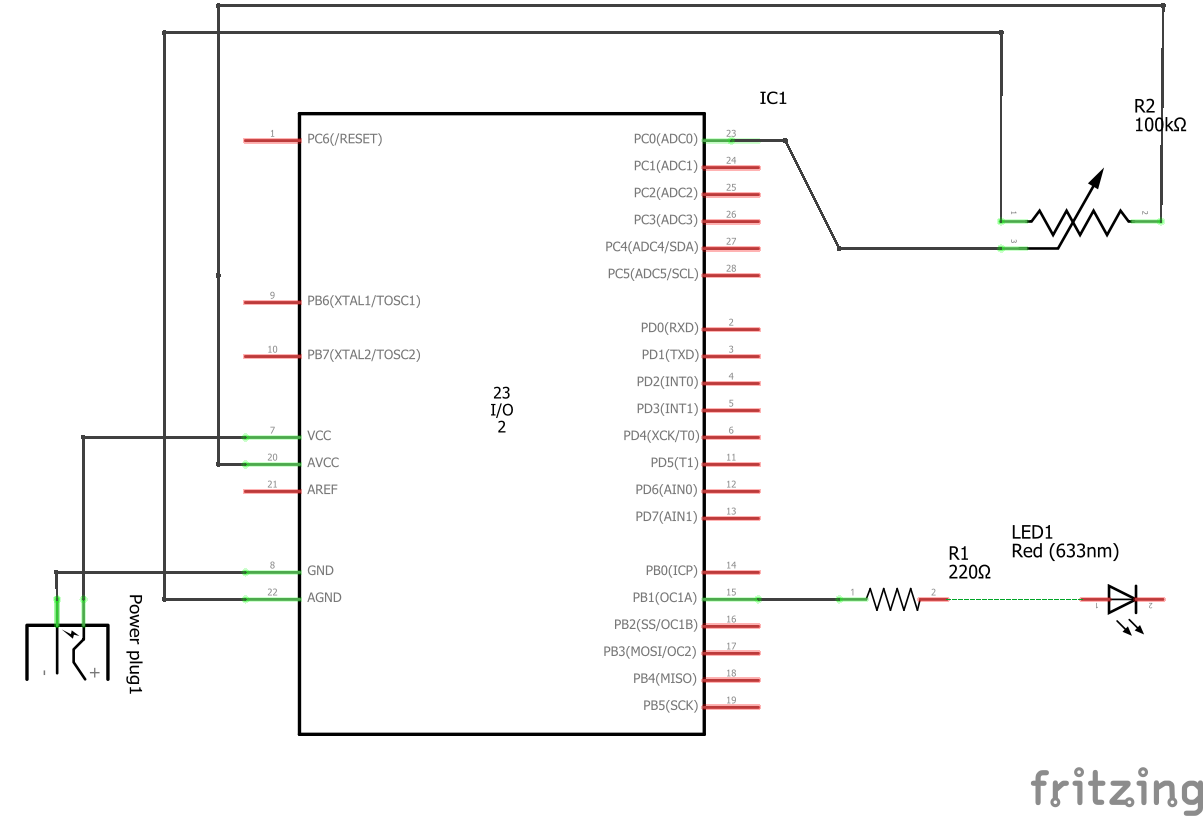
\includegraphics[scale=0.8]{esquema_fading.png}
 \fautor
\end{figure}

Veja também o circuito montado na protoboard na figura 3:

 \begin{figure}[htb]
 \caption{Montagem: Fading LED}
 \label{fig:Montagem Fading LED}
 \centering
 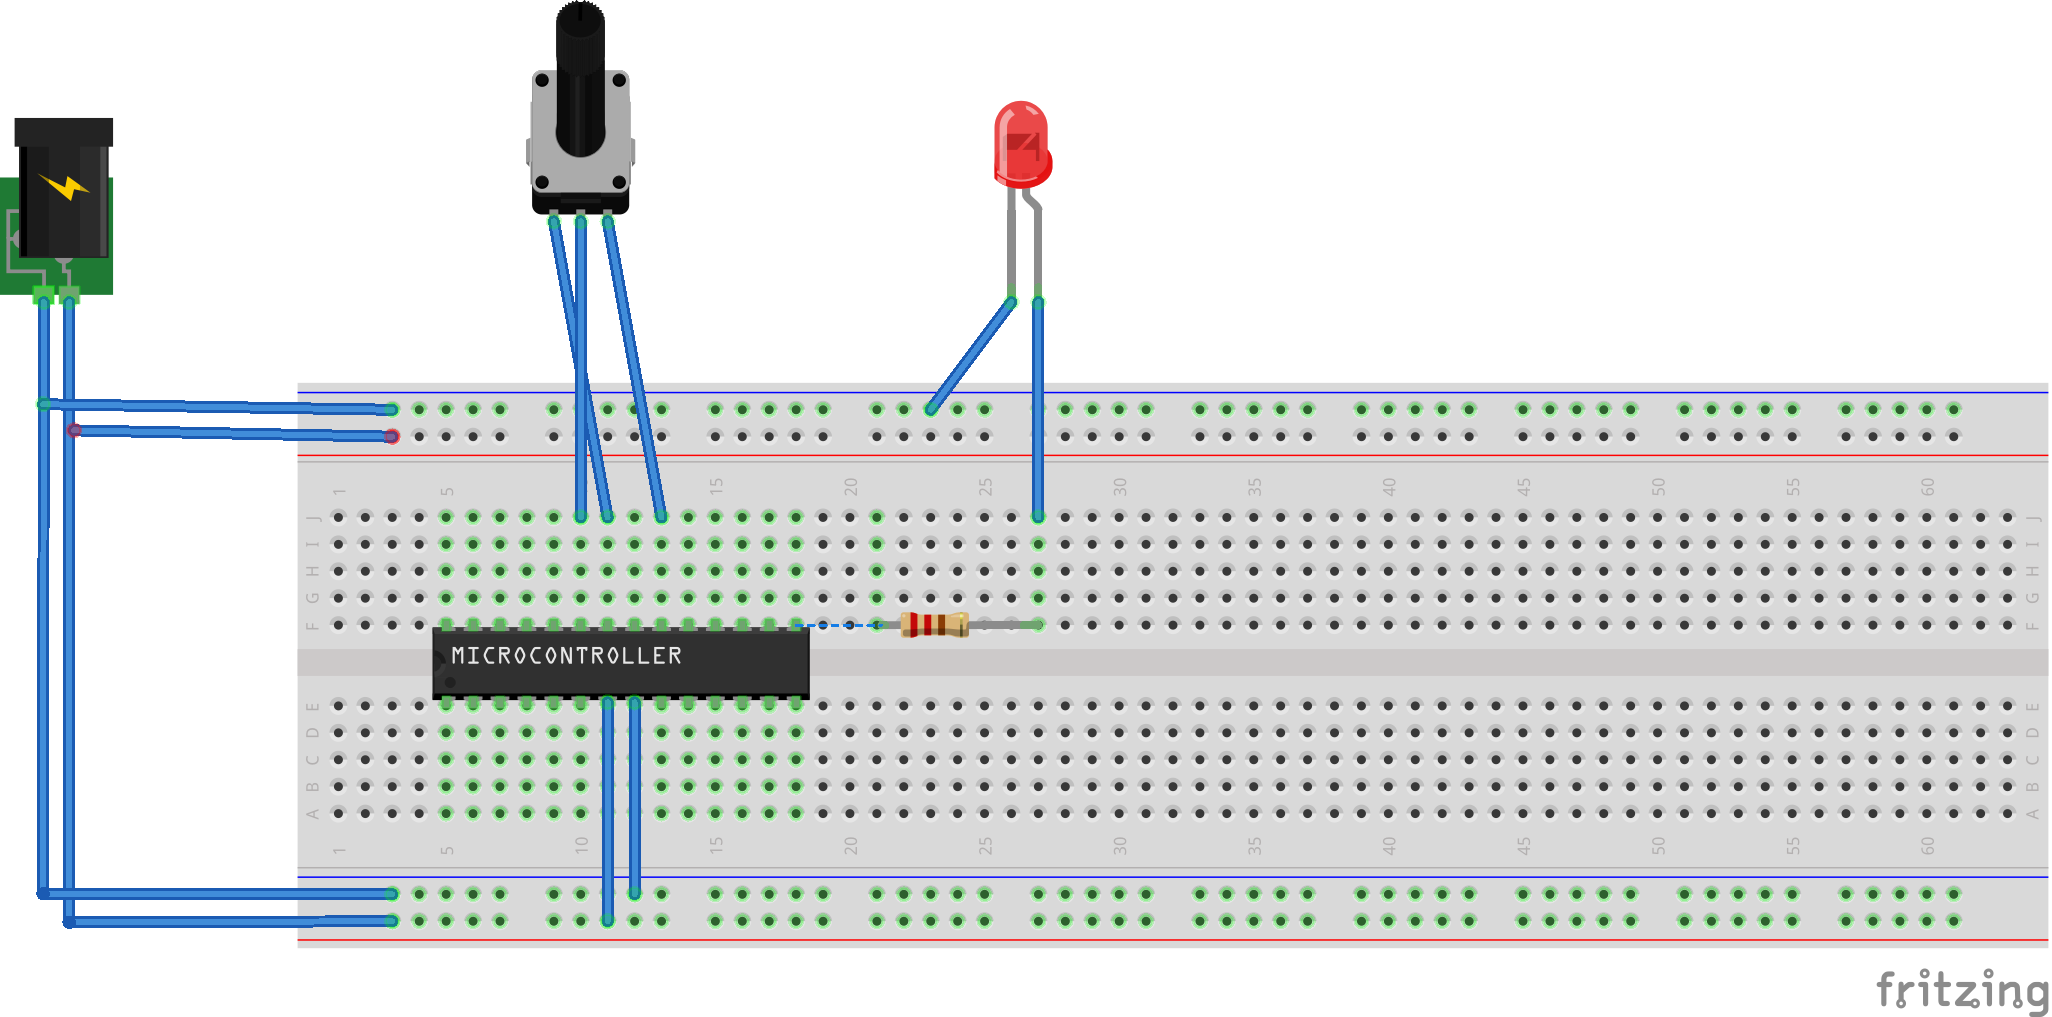
\includegraphics[scale=0.5]{montagem_fading.png}
 \fautor
\end{figure}

\section{Código em C}

%\begin{algoritmo}
%\caption{Algoritmo para cálculo de máximo divisor comum MDC($n_1$,$n_2$)}
%\label{algoritmo:mdc1}
%
% \KwIn{Dois números inteiros ($n_1, n_2$)}
% \If(\tcp*[f]{Garante que o maior número seja $n_1$}){$n_2 > n_1$}
%   {troca valores de $n_1$ e $n_2$}
% \Repeat{$r > 0$}{
%    $r \leftarrow$ resto da divisão de $n_1$ por $n_2$
%    $n_1 \leftarrow n_2$
%    $n_2 \leftarrow r$
% }
% \Return $n_1$
%\end{algoritmo}

\begin{codigo}[caption = {Fading LED}, label={codigo:fading LED},language=C, breaklines=true]
 
  /*******************************************************************
 *      Fading Led
 *
 * Universidade Federal de Goiás
 * Microcontrolador Utilizado: AVR ATMega8
 * Grupo: Marco Túlio / Vitor do Vale Bernardo / Pablo Silva
 * Descrição: O codigo recebe os valores lido na entrada PWM atráves de um/
 *		   	  Potênciometro e irá ligar o LED proporcionalmente.
 * 
 ********************************************************************/

#define FOSC 1000000UL// Clock Speed
#define BAUD 1200
#define MYUBRR ((FOSC/ (BAUD * (long)16)))

#include <avr/io.h>
#include <util/delay.h>
#include <util/setbaud.h>
#include <avr/eeprom.h>
#include <avr/interrupt.h>

void USART_Init( unsigned intubrr);
void USART_Transmit(unsigned char data);
unsigned char USART_Receive(void);
uint16_t ReadADC(uint8_t ch);
void InitADC();


int main(void)
{
	
	//PWM Initialisation
	TCCR1A = 0b10000001; // fast PWM mode 8-bit on OC1A
	TCCR1B = 0b00001010; // prescaling by 8
	
	//Initial value;
	OCR1A = 0x00;
	DDRB = 0xFF; // set port B for output


	unsigned char lei;
	InitADC();
	USART_Init(MYUBRR);
	while(1)
	{
		OCR1A =ReadADC(0);
		_delay_ms(10);
	}
}

void USART_Transmit(unsigned char data)
{
	while( !( UCSRA & (1<<UDRE)) );
	UDR = data;
}


void USART_Init(unsigned int ubrr)
{
	UBRRH=(unsigned char)(ubrr>>8);
	UBRRL=(unsigned char)ubrr;
	UCSRB=(1<<RXEN)|(1<<TXEN);
	UCSRC=(1<<URSEL)|(1<<USBS)|(3<<UCSZ0);
}

unsigned char USART_Receive(void)
{
	while(!(UCSRA & (1<<RXC)));
	return UDR;
}


void InitADC()
{
	ADMUX=(1<<REFS0);             // For Aref=AVcc;
	ADCSRA=(1<<ADEN)|(1<<ADPS2)|(1<<ADPS1)|(1<<ADPS0); //Rrescalar div factor =128
}


uint16_t ReadADC(uint8_t ch)
{
	
	//Seleciona o canal de leitura do microcontrolador
	ch=ch&0x07;
	ADMUX|=ch;
	//inicia a conversão
	ADCSRA|=(1<<ADSC);
	//Aguarda a conversão
	while(!(ADCSRA & (1<<ADIF)));
	//Limpa a flag
	ADCSRA|=(1<<ADIF);
	//retorna o dado
	return(ADC);
}

\end{codigo}

\chapter{Proejeto 2: Sleep Mode}
\label{chapter:Sleep Mode}

Desenvolva um projeto que desligue um LED e mantenha desligado em um determinado período de tempo. No período em que o LED estiver
desligado, todo o sistema deve entrar em sleep mode. Depois de um determinado tempo, o sistema deve ser ativado e ligar o LED novamente.


\section{O que é Sleep Mode?}

Podemos utilizar a instrução SLEEP para reduzir fortemente o consumo de energia por uma determinada aplicação. Os dispositivos AVR podem ser colocados em diferentes modos de sleep, neste caso o dispositivo AVR que estamos trabalhando é ATMega8.

A biblioteca sleep.h possui diferentes macros para colocar o dispositivo em modo de suspensão. A forma mais simples é opcionalmente configurando o modo de suspensão desejado utilizando a função: Set Sleep Mode, (O padrão é o modo ocioso  onde que CPU é coloca no modo de suspensão, mas todos os relógios e periféricos ainda estão em execução) e em seguida devemos ativar o modo de sleep usando a função: sleep_mode.

\section{Esquemático e Montagem}

Este projeto tem como objetivo simular o uso do “sleep mode” em um circuito. Quando este modo está ativado, todo o sistema fica em espera, com um baixo uso de recursos, aguardando para voltar ao estado normal quando requisitado. Para o auxílio do projeto, será utilizado um LED para sinalizar quando o sistema entrou e saiu de fato do “sleep mode”. O LED ligado indica que o sistema está operando normalmente. Ao desligar o LED, o sistema deve então simultaneamente entrar em “sleep mode” durante um tempo determinado previamente. Após o fim desse tempo, o sistema então retornará ao seu estado normal e o LED deve ser religado.

\begin{figure}[htb]
 \caption{Esquemático: Sleep Mode}
 \label{fig:Esquemático: Sleep Mode}
 \centering
 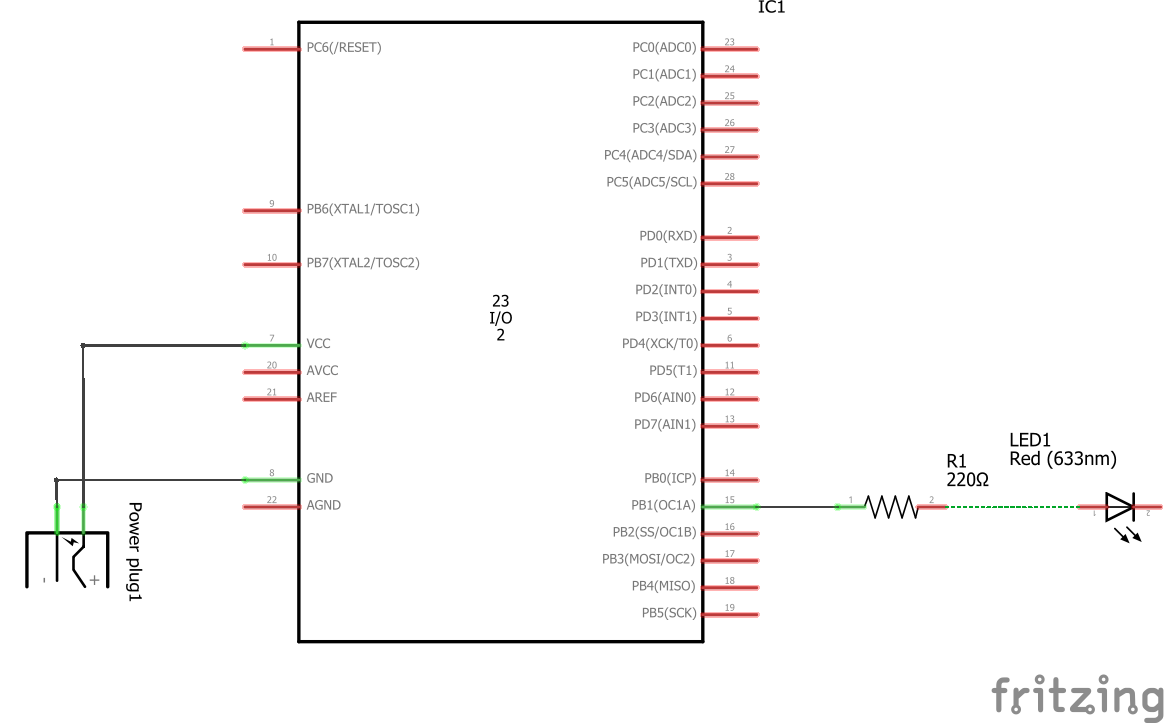
\includegraphics[scale=0.8]{SleepMode_esquematico.png}
 \fautor
\end{figure}

\begin{figure}[htb]
 \caption{Montagem: Sleep Mode}
 \label{fig:Montagem: Sleep Mode}
 \centering
 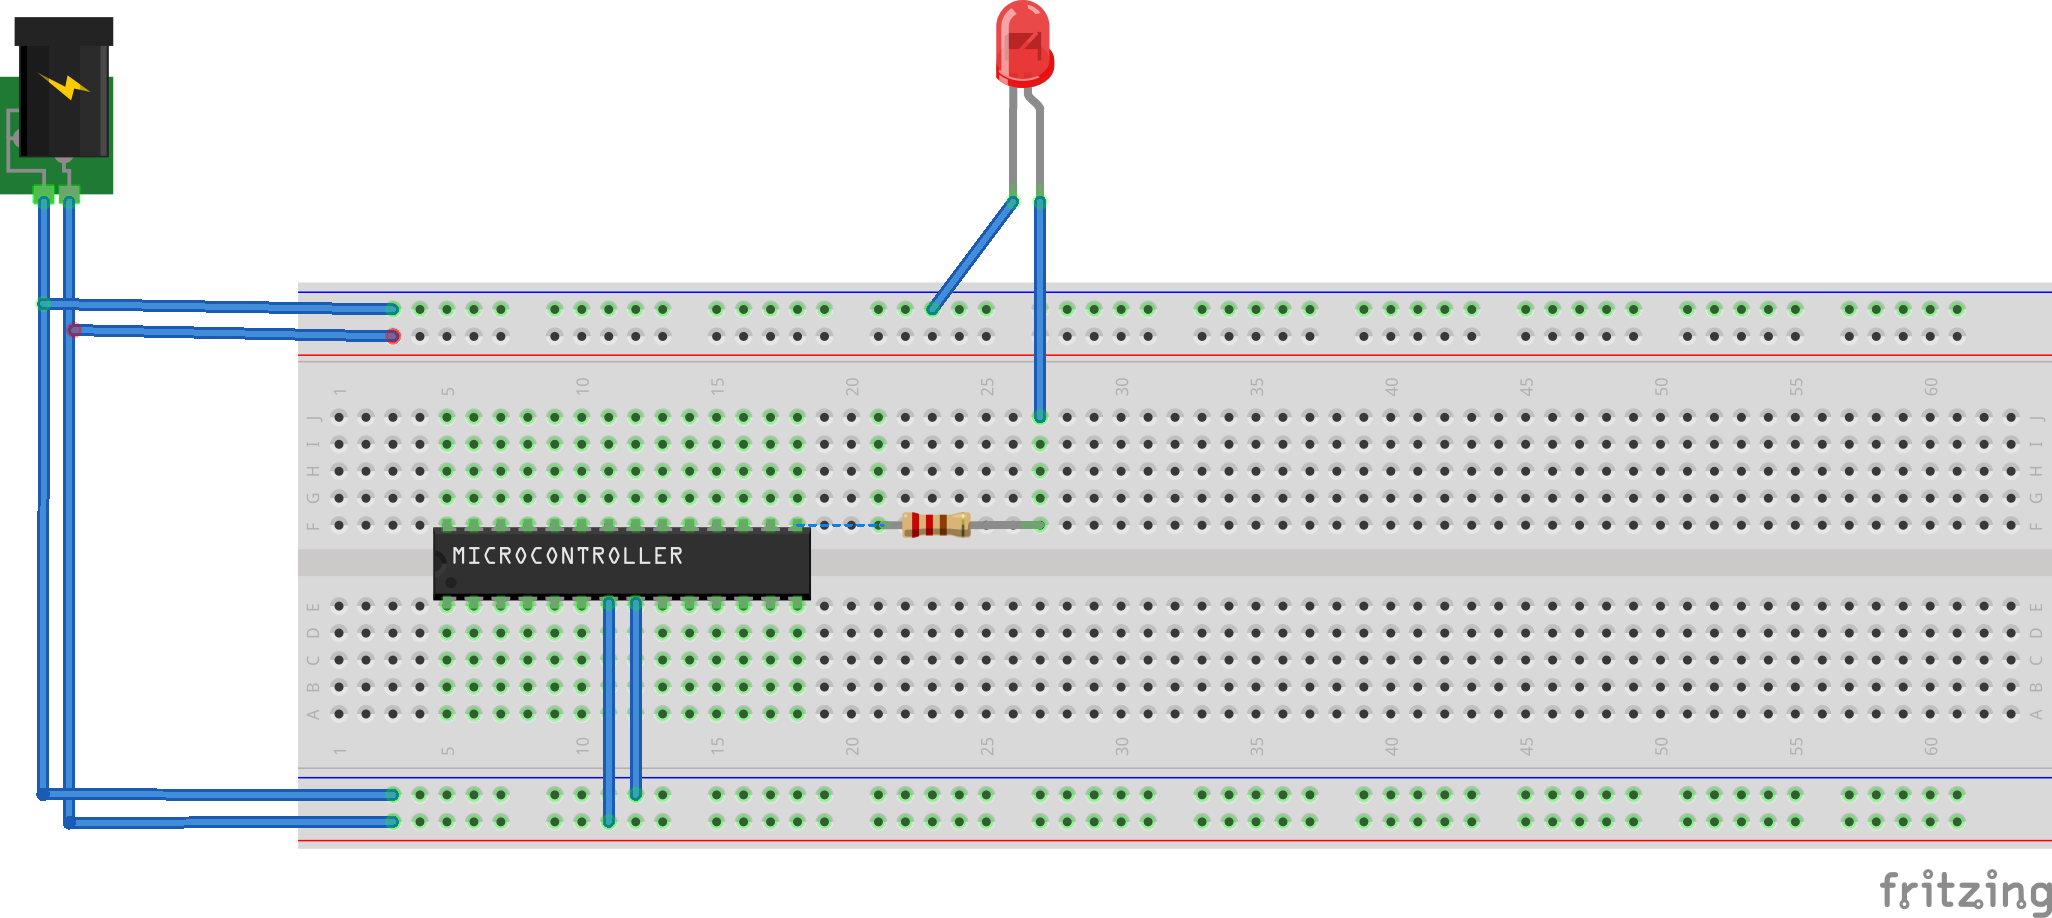
\includegraphics[scale=0.8]{SleepMode_montagem.png}
 \fautor
\end{figure}

\begin{codigo}[caption = {Led On/Off in Sleep Mode}, label={codigo: Led On/Off with Slep Mode},language=C, breaklines=true]

 
 /**************************************************************************
 *      Led On/Off - Utlizando Sleep Mode
 *
 * Universidade Federal de Goiás
 * Microcontrolador Utilizado: AVR ATMega8
 * Grupo: Marco Túlio / Vitor do Vale Bernardo / Pablo Silva
 * Descrição: Ligar e desligar um LED utilizando o modo sleep.
 * 
 ************************************************************************/

#include <avr/io.h>
#include <avr/sleep.h>
#include <avr/interrupt.h>
#include "util/delay.h"

int main(void)
{
	DDRB = 0xFF;

   // infinite main loop
   while (1)
   {
	
	PORTB = 0x01; //  Liga Led na porta 01
	_delay_ms(2000); // Espera 2 segundo
	set_sleep_mode(SLEEP_MODE_PWR_SAVE);
	cli(); 	// desligar interrupções
	sleep_enable();	 // Ativa o Sleep Mode
	sei(); //Liga as interrupções
	sleep_cpu(); 
	cli();
	_delay_ms(5000);
	sleep_disable();
	sei();
	
   }
   
}

\end{codigo}

\chapter{Proejeto 3: Comunicação SPI}
\label{chapter: Comunicação SPI}
Desenvolva um projeto que realize a comunicação entre dois microcontroladores utilizando o padrão SPI.

\section{O que é o Padrão SPI?}

Neste trabalho iremos mostrar uma das diversas tecnologias diferentes existentes para fazer a comunicação serial entre dois dispositivos. Durante o discorrer deste estaremos trabalhando com o padrão \sigla{SPI}{Serial Peripheral Interface}.

Na comunicação serial síncrona definimos também o conceito de Mestre-Escravo. Normalmente o gerador do sinal de sincronismo é definido como o Mestre (Master) da comunicação. Para os dispositivos que utilizam do sinal de sincronismo gerado damos a definição de Escravo (Slave). A ligação mais comum desse tipo de comunicação é um Master e vários Slaves.

\begin{figure}[htb]
 \caption{Master and Slaves}
 \label{fig:Master and Slaves}
 \centering
 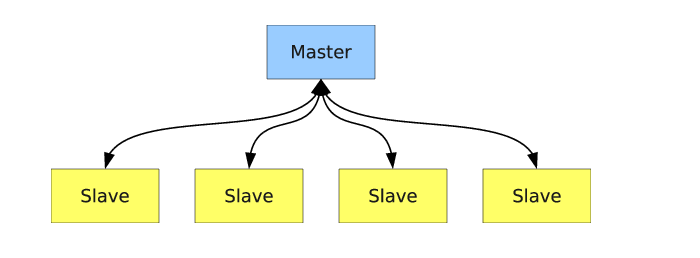
\includegraphics[scale=0.5]{Master_And_Slave.png}
 \fdireta{embarcados:master_slave}
\end{figure}

Os pinos básicos de comunicação entre dispositivos utilizando o protocolo SPI e o esquema padrão de ligação são dados conforme abaixo:

\begin{figure}[htb]
 \caption{Pinos do SPI}
 \label{fig:Pinos para comunicação SPI}
 \centering
 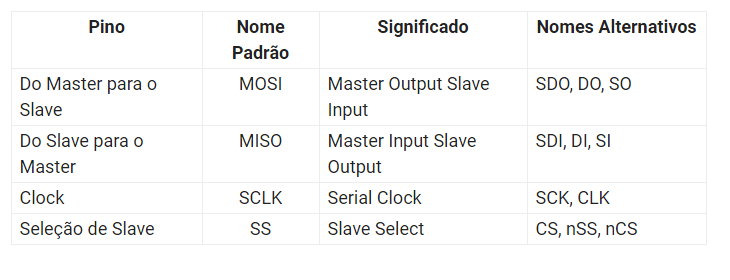
\includegraphics[scale=0.5]{pinos.png}
 \fdireta{embarcados:master_slave}
\end{figure}

O sinal de SS funciona como Seleção de Escravo (Slave Select). É um sinal ativo em nível baixo, o que significa que o dispositivo é selecionado quando este pino se encontra em nível baixo. No entanto, muitos dispositivos utilizam este sinal como sincronismo de frame. Dessa forma, é um sinal importante que deve ser respeitado.

\section{Esquemático e Montagem}

Neste projeto realizaremos a comunicação entre dois microcontroladores distintos com o uso do padrão \sigla{SPI}{Serial Peripheral Interface}, que trata-se de um protocolo que permite a comunicação de um microcontrolador com diversos outros componentes, formando uma rede. Os dois microcontroladores utilizados serão identificados por mestre e escravo (master / slave). O mestre será encarregado de enviar os comandos através da comunicação serial, enquanto o escravo é encarregado de receber, interpretar e executar uma determinada ação com base nos dados recebidos. Os comandos enviados de um microcontrolador são um indicador de qual será o estado de um LED, ligado ou desligado.

Veja o esqumático na imagem abaixo: 

\begin{figure}[htb]
 \caption{SPI: Esquemático da montagem}
 \label{fig:SPI: Esquemático da montagem}
 \centering
 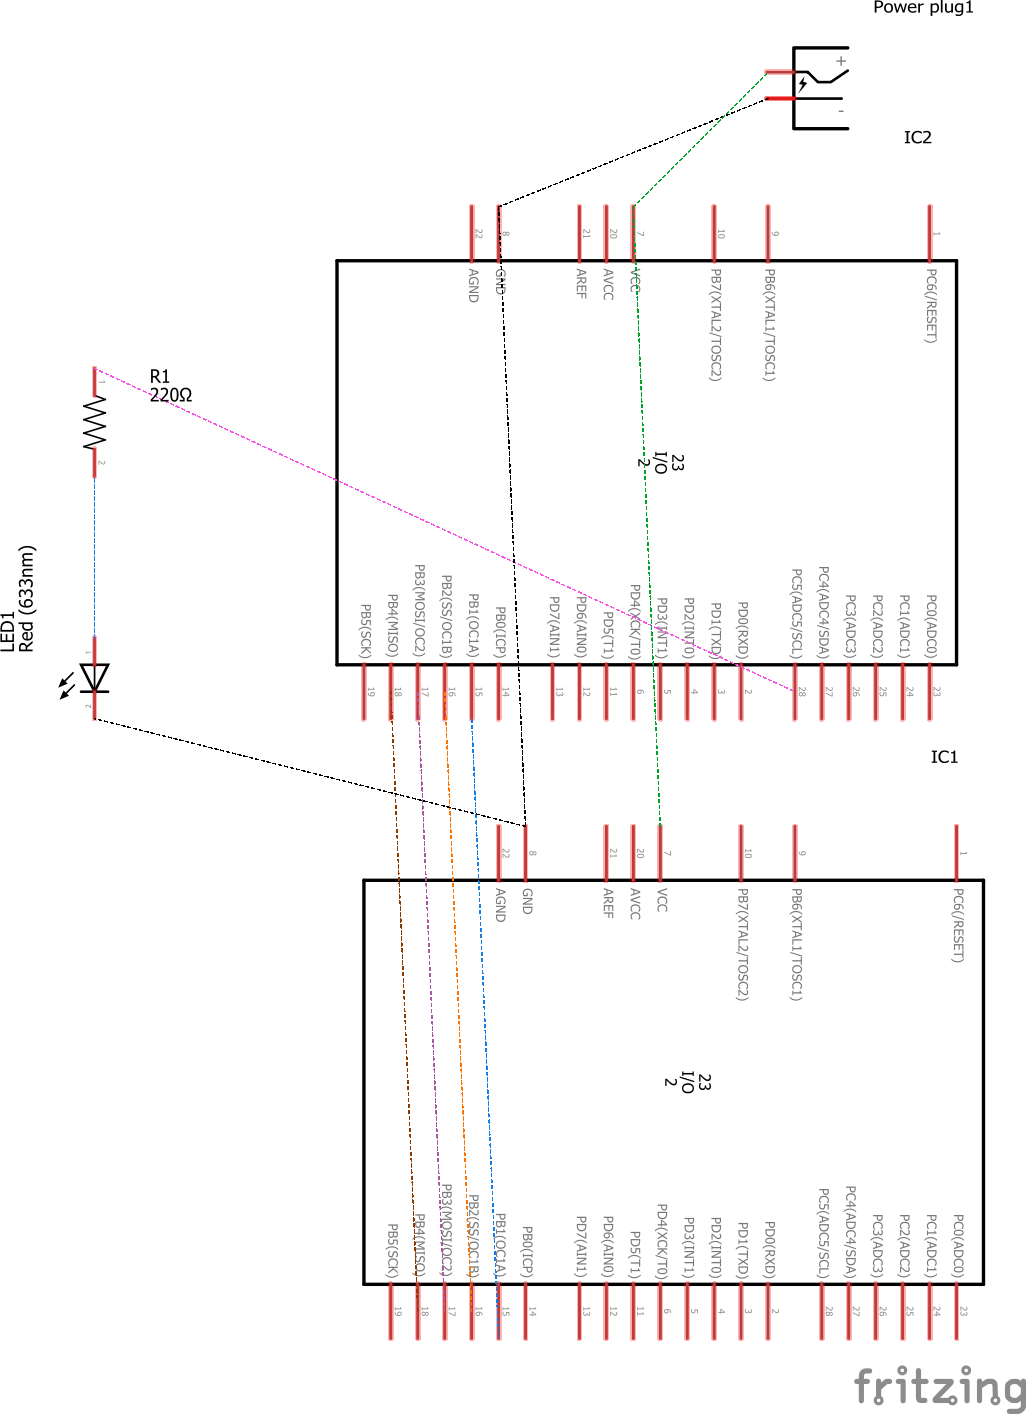
\includegraphics[scale=0.5]{SPI_esquematico.png}
 \fautor
\end{figure}

\begin{figure}[htb]
 \caption{SPI: Montagem na Protoboard}
 \label{fig:SPI: Montagem na Protoboard}
 \centering
 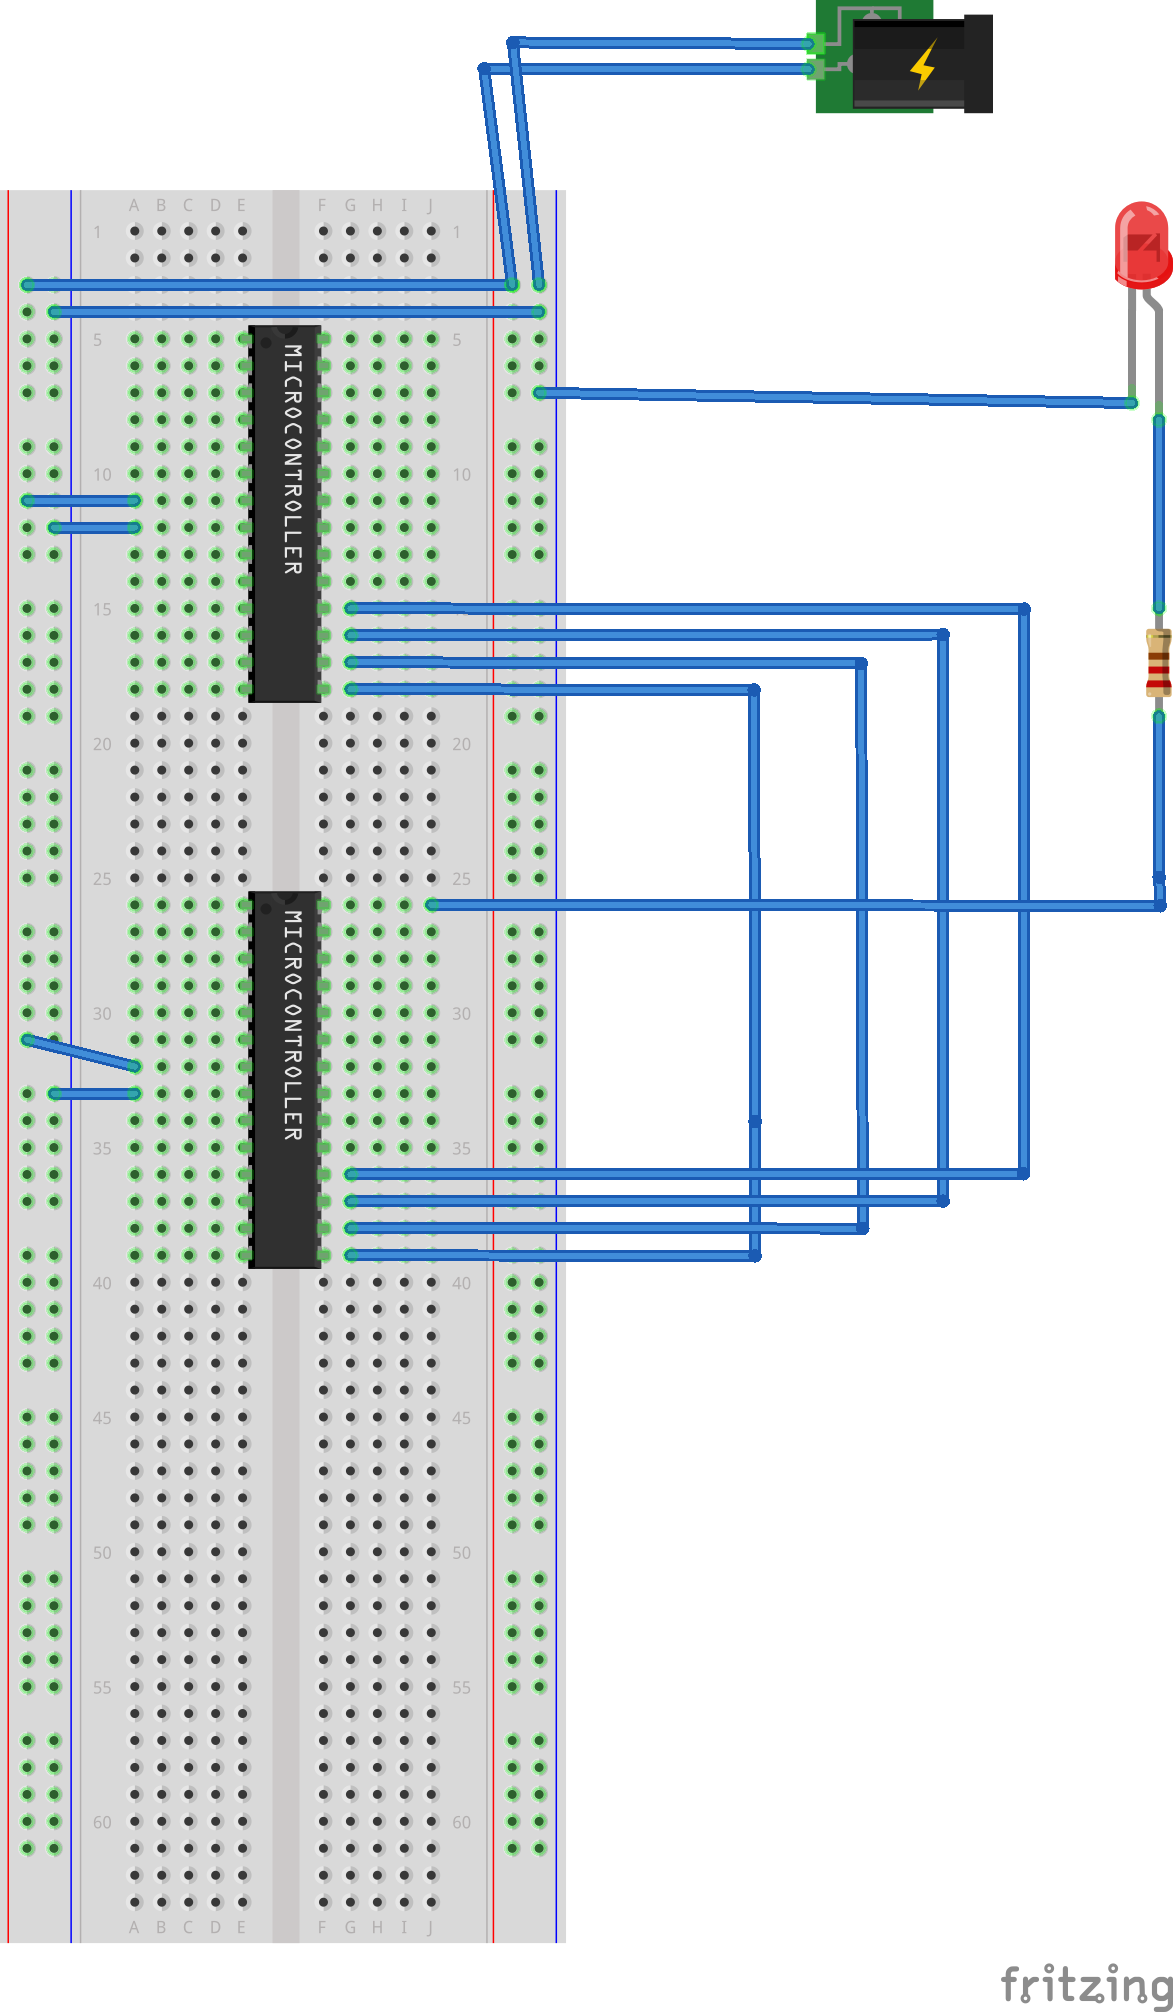
\includegraphics[scale=0.5]{SPI_montagem.png}
 \fautor
\end{figure}

\section{Código em C}

O código para este projeto é dividio em duas partes: Código do Master e o Código do Slave.

\begin{codigo}[caption = {MASTER - Comunicação via SPI entre dois dispositivos}, label={codigo: Comunicação entre dispositivos AVR usando SPI - MASTER },language=C, breaklines=true]

 /**************************************************************************
 *      Comununicação entre dois Microcontroladores Utilizando  SPI (Master)
 *
 * Universidade Federal de Goiás
 * Microcontrolador Utilizado: AVR ATMega8
 * Grupo: Marco Túlio / Vitor do Vale Bernardo / Pablo Silva
 * Descrição: Codigo Master irá enviar comandos pela comunicação SPI para o slave
 *            O comando ira dizer o estado do LED: ligado ou desligado.
 * 
 ************************************************************************/
    

#define F_CPU 4000000UL           // clock do microcontrolador
#include <avr/io.h>
#include <util/delay.h>
#include <avr/interrupt.h>
 
/////////////////////////////configuração dos pinos utilizados //////////////////////////////////////
 
#define MOSI         PB3
#define MISO         PB4
#define SCK          PB5
#define SS           PB2
 
/////////////////////////////////////////////////////////////////////////////////////////////////////////
  void SPI_inicializa(void)
  {
      DDRD =0xFF;
      DDRB |= ((1<<MOSI)|(1<<SCK)|(1<<SS));    //MOSI, SCK and SS são saidas(se for usar dois mestres então deve-se o SS como entrada) 
      DDRB &= (~(1<<MISO));                    //MISO é entrada
      PORTB |= (1<<SS);                        //inicia com SS em nivel alto
      //SPE : habilita SPI
      //MSTR: modo  Master 
      //SPIE:  habilita interrupção de SPI
      //SPCR = ((1<<SPE)|(1<<MSTR)|(1<SPR1)|(1<SPR0));    //(1<SPR1)|(1<SPR0) : FOSC/128
      SPCR = ((1<<SPE)|(1<<MSTR)|(1<SPR0));    //(1<SPR0) : FOSC/16
  }
   
  void SPI_envia_byte(char dados)
  {
      PORTB &= (~(1<<SS));    //coloca SS em nivel baixo (0), para transferir dados
      SPDR = dados;        //inicializa transferencia
      while(!(SPSR & (1<<SPIF)));    //espera fim de transmissão
      PORTD = SPDR;//escreve no port D o dado recebido
      PORTB |= (1<<SS);    //coloca SS em nivel alto (1), pois é o fim da transmissão.
      _delay_ms(1);//tempo para slave colocar dados no registrador
  }
   
  int main(void) 
  {
    
    SPI_inicializa();//inicializa SPI
    sei();//habilita interrupções
   
    while(1)
	{
      SPI_envia_byte(0X01); /*** Envia o primeiro comando: LIGAR LED***/
      _delay_ms(1000); /*** Delay de 1 segundo ***/
	   SPI_envia_byte(0x00); /*** Envia o segundo comando: DESLIGAR LED ***/
	   _delay_ms(1000);  /*** Delay de 1 segundo ***/
  }
   
    return 0;
  }

\end{codigo}


\begin{codigo}[caption = {SLAVE - Comunicação via SPI entre dois dispositivos}, label={codigo: Comunicação entre dispositivos AVR usando SPI - SLAVE },language=C, breaklines=true]

 
 /**************************************************************************
 *      Comununicação entre dois Microcontroladores Utilizando  SPI (Slave)
 *
 * Universidade Federal de Goiás
 * Microcontrolador Utilizado: AVR ATMega8
 * Grupo: Marco Túlio / Vitor do Vale Bernardo / Pablo Silva
 * Descrição: Codigo Slave irá receber os dados enviados pelo Master e colocara no PORTD,
 *            Ligando e desligando o LED.
 * 
 ************************************************************************/
    
   #define F_CPU 4000000UL  // Definindo o Clock do Microcontrolador
   #include <avr/io.h>
   #include <avr/interrupt.h>
   
   /*********************************
   *	Definindo os Registradores  *
   *********************************/
   
   #define MOSI     PINB3 /*******Definindo o PINB3 como entrada********/
   #define MISO     PINB4 /********Definindo o PINB4 como saída********/
   #define SCK      PINB5 /********Definindo o PINB5 como entrada********/
   #define DDR_SPI  DDRB
    
   char enviar=0;
    
   /*********************************
   *	Inicializando			    *
   *********************************/
   
   void SPI_Slave_inicializa(void)
   {
       DDR_SPI = (1<<MISO);
       SPCR = (1<<SPE)/*|(1<<CPOL)*/|(1<<SPIE); /****Aviva o SPI / polaridade do clock / habilita interrupção de SPI ****/
   }
   
   /**** Vetor de Interrupção *****/
   ISR (SPI_STC_vect)                         
   {
     SPDR = enviar; //envia dado anteriormente recebido
     PORTD = SPDR;
	 PORTC = SPDR;
     enviar = SPDR;
   }
   
   /*********************************
   *	Função Principal		    *
   *********************************/
   int main(void) 
   { 
       SPI_Slave_inicializa();
       DDRD = 0xFF;
       DDRC = 0XFF;
	   sei();
	   
	   while(1){
		   
	   }

   }

\end{codigo}





















% ---
% Finaliza a parte no bookmark do PDF, para que se inicie o bookmark na raiz
% ---
\bookmarksetup{startatroot}% 
% ---

% ----------------------------------------------------------
% ELEMENTOS PÓS-TEXTUAIS
% ----------------------------------------------------------
\postextual

% ----------------------------------------------------------
% Referências bibliográficas
% ----------------------------------------------------------
\bibliography{references}

% ---------------------------------------------------------------------
% GLOSSÁRIO
% ---------------------------------------------------------------------

% Arquivo que contém as definições que vão aparecer no glossário
\newword{WYSIWYG}{``What You See Is What You Get''  ou ``O que você vê é o que você obtém''.  Recurso tem por objetivo permitir que um documento, enquanto manipulado na tela, tenha a mesma aparência de sua utilização, usualmente sendo considerada final. Isso facilita para o desenvolvedor que pode trabalhar visualizando a aparência do documento sem precisar salvar em vários momentos e abrir em um \textit{software} separado de visualização}
\newword{Framework}{é uma abstração que une códigos comuns entre vários projetos de \textit{software} provendo uma funcionalidade genérica. \textit{Frameworks} são projetados com a intenção de facilitar o desenvolvimento de \textit{software}, habilitando designers e programadores a gastarem mais tempo determinando as exigências do \textit{software} do que com detalhes de baixo nível do sistema}

\newword{Template}{é um documento sem conteúdo, com apenas a apresentação visual (apenas cabeçalhos por exemplo) e instruções sobre onde e qual tipo de conteúdo deve entrar a cada parcela da apresentação}

\newword{Padrões de projeto}{ou \textit{Design Pattern}, descreve uma solução geral reutilizável para um problema recorrente no desenvolvimento de sistemas de \textit{software} orientados a objetos. Não é um código final, é uma descrição ou modelo de como resolver o problema do qual trata, que pode ser usada em muitas situações diferentes}

\newword{Web}{Sinônimo mais conhecido de \textit{World Wide Web} (WWW). É a interface gráfica da Internet que torna os serviços disponíveis totalmente transparentes para o usuário e ainda possibilita a manipulação multimídia da informação}

% Comando para incluir todas as definições do arquivo glossario.tex
\glsaddall
% Impressão do glossário
\printglossaries

% ----------------------------------------------------------
% Apêndices
% ----------------------------------------------------------

% ---
% Inicia os apêndices
% ---

% ---


% ----------------------------------------------------------
% Anexos
% ----------------------------------------------------------

% ---
% Inicia os anexos
% ---
% ---

\end{document}